\section{SPI slave block}
\label{sec:SPIslaveblock}
This section will describe in detail how the SPI slave in the FPGA receives and transmits data, according to the description of the SPI communication protocol mentioned before.

\subsection{Description}

The SPI slave has two different tasks. The first task is to exchange data with the SPI master in the microcontroller. The second task is to store the information that is received and present it to the components that need the data. The SPI slave could be called also some sort of information bank for the driver.\\
The data exchange part follow the SPI communication protocol mentioned in section \ref{sec:SPIcommunication}.
The information bank part is made by having the block hold the information in the actual output of the block. This is done so that the data is constantly supplied to the block in need of the data. However this requires a lot of data paths, but this is not much of a problem since this is going on internally in the FPGA. The reason the data is stored in the SPI slave component was also to make it more manageable, since all of the data is stored at the same place.

\subsection{Implementation}
\label{sec:Implementation}
The SPI slave could have been implemented as a state machine. However because of the rather simplistic nature of the SPI communication protocol it was chosen not to implement it as a state machine. Instead it was implemented as a series of different events that trigger different responses in the SPI block. The first event is the S\_CLK pin is having an rising edge. This event makes the the SPI slave read the input from the MOSI pin and prepare the next output for the MISO pin. The code that handles this event can be seen in figure \ref{fig:S_CLK_code_example}. 

\begin{figure}[h!]
\centering
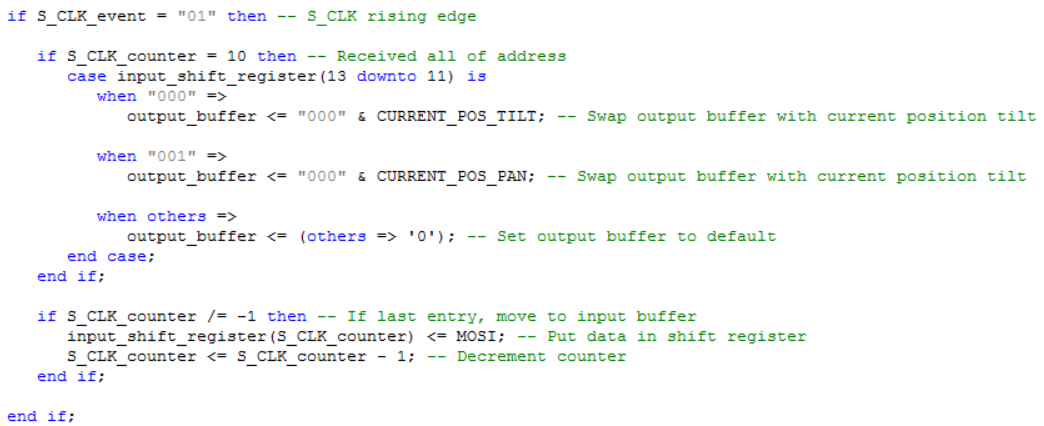
\includegraphics[scale=0.5]{Billeder/FPGA/SPI_Slave/S_CLK_code_example.png}
\caption{ An S\_CLK code example }
\label{fig:S_CLK_code_example}
\end{figure}

\newpage

The second event is when the SS pin has a rising edge. This signifies that the transmission is over and that all of the packet should be sent. This event triggers the SPI slave to update the data received on the correct output according to the received address for the data. An example of the code doing this can be seen in figure \ref{fig:SS_code_example}.

\begin{figure}[h!]
\centering
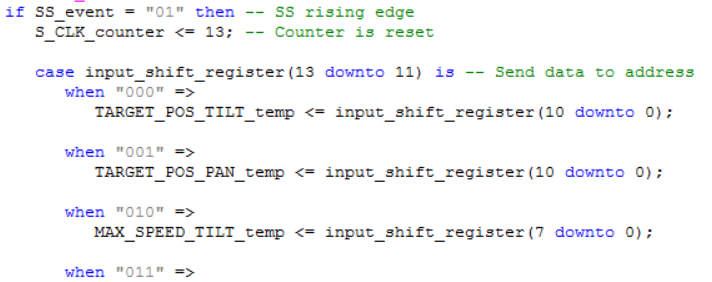
\includegraphics[scale=0.5]{Billeder/FPGA/SPI_Slave/SS_code_example.png}
\caption{ An SS code example }
\label{fig:SS_code_example}
\end{figure}

During the data transaction, two temporary registers are used, one for the input and one for the output. This is done to stabilize the data send so that it does not change mid transmission which would cause the data to become corrupt.
There are 4 different kinds of settings that can be controlled via the SPI slave. The first setting is the target position used in the controller block, the second setting is the maximum speed for the motor, the third setting is the minimum speed of the motor and the last setting is the enabling of the motor. All of these 4  settings can be set for the pan and tilt part separately. This results in 8 different values needing an address resulting in an address length of 3 bits.
Since the data length has to be constant, the data length was chosen according to the largest value needed to be sent. This was the target position, needing 11 data bits hence the data length was chosen to be 11 bits. 

The output from the SPI slave to the SPI master was chosen to mimic the address and then send some data according to the address received under the transmission. This means that the output buffer has to be changed under the transmission. This would be a problem in most cases, however since the FPGA works much faster than the microcontroller this is not a problem. Since the only information the SPI master is interested in is the current position, the output buffer is only changed when this information is polled. It was made so that this information was always polled when a target position was sent, meaning that if only a poll on the current position is wanted. the target position is resent with the same value. In all other scenarios than the master sending the target position, the value returned to the master is the address the master sent and a data containing zeroes. The code handling this can also be seen in \ref{fig:S_CLK_code_example}.

\subsection{Tests}

The SPI slave component has been tested in a Xillinx ISE testbench. This was done by simulating a transaction to the SPI slave. In figure \ref{fig:Pos_change_testbench} the test bench can be seen. SS can be seen going low signifying the start of the data transfer.

The S\_CLK then starts to toggle and the data is shifted into the input register and as SS goes high the data from the input register is set to the placement the address is pointing to. In this case, a value to the target of the pan is being send. This has the address of 001 which can also be seen on the three first bits in the input register.

\begin{figure}[h!]
\centering
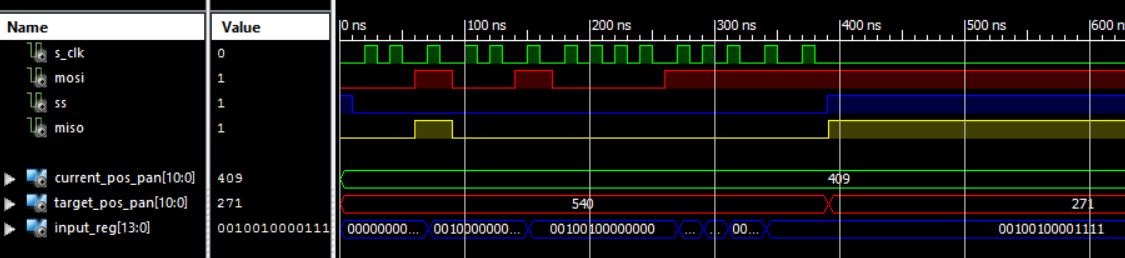
\includegraphics[scale=0.5]{Billeder/FPGA/SPI_Slave/Testbench_of_SPI.png}
\caption{ An Xilinx testbench simulation of the SPI }
\label{fig:Testbench_of_SPI}
\end{figure}

\subsection{Discussion}

One of the features you would get from creating the SPI slave component as a state machine is more robustness against errors. When an error happens in a state machine it would be unable to make the same amount of mess because it is locked to the state. However since no error should be happening and the fact that at no time while testing the connection was an error made, it is not really of any concern.

\subsection{Conclusion}

Both the testbench and physical test with the FPGA and microcontroller showed that this component functioned as it should.